\documentclass[8pt]{extarticle}
\title{}
\author{Avinash Iyer}
\date{}
\usepackage[shortlabels]{enumitem}

%font setup
%
\usepackage{newpxtext,eulerpx}

%paper setup
\usepackage{geometry}
\geometry{letterpaper, portrait, margin=1in}
\usepackage{fancyhdr}

%symbols
\usepackage{amsmath}
\usepackage{mathtools}
\usepackage{hyperref}
\usepackage{gensymb}

\usepackage[T1]{fontenc}
\usepackage[utf8]{inputenc}

\usepackage[version=4]{mhchem}
\usepackage{chemfig}

%plotting
\usepackage{pgfplots}
\usepackage{tikz}
\tikzset{middleweight/.style={pos = 0.5, fill=white}}
\tikzset{weight/.style={pos = 0.5, fill = white}}
\tikzset{lateweight/.style={pos = 0.75, fill = white}}
\tikzset{earlyweight/.style={pos = 0.25, fill=white}}

%\usepackage{natbib}

%graphics stuff
\usepackage{graphicx}
\graphicspath{ {./images/} }

%code stuff
%when using minted, make sure to add the -shell-escape flag
%you can use lstlisting if you don't want to use minted
%\usepackage{minted}
%\usemintedstyle{pastie}
%\newminted[javacode]{java}{frame=lines,framesep=2mm,linenos=true,fontsize=\footnotesize,tabsize=3,autogobble,}
%\newminted[cppcode]{cpp}{frame=lines,framesep=2mm,linenos=true,fontsize=\footnotesize,tabsize=3,autogobble,}

\usepackage{listings}
\usepackage{color}
\definecolor{dkgreen}{rgb}{0,0.6,0}
\definecolor{gray}{rgb}{0.5,0.5,0.5}
\definecolor{mauve}{rgb}{0.58,0,0.82}

\lstset{frame=tb,
	language=Java,
	aboveskip=3mm,
	belowskip=3mm,
	showstringspaces=false,
	columns=flexible,
	basicstyle={\small\ttfamily},
	numbers=none,
	numberstyle=\tiny\color{gray},
	keywordstyle=\color{blue},
	commentstyle=\color{dkgreen},
	stringstyle=\color{mauve},
	breaklines=true,
	breakatwhitespace=true,
	tabsize=3
}
% text + color boxes
\usepackage{tcolorbox}
\tcbuselibrary{breakable}
\newtcolorbox{problem}[1]{colback = white, title = {#1}, breakable}
\newtcolorbox{solution}{colback = white, colframe = black!75!white, title = Solution, breakable}
%including PDFs
\usepackage{pdfpages}
\setlength{\parindent}{0pt}

\pagestyle{fancy}
\fancyhf{}
\rhead{Avinash Iyer}
\lhead{Econ 308: Class Notes}
\begin{document}{
  \begin{problem}{Introduction to Public Economics}
    Governments play a crucial role in much economic life.
    \begin{itemize}
      \item Regulatory structure (financial markets, pharmaceuticals, labor markets, civil rights).
      \item Taxes.
      \item Public goods and social welfare spending.
      \item Macroeconomic stabilization.
    \end{itemize}
   Public finance is the study of the role of government in a market economy, primarily focusing on taxes and spending.\\

   Reasons to study public economics:
    \begin{itemize}
      \item Governments have a lot of power in the realm of economic welfare.
      \item Nearly every economic transition is mediated by the government.
      \item It can inform debates about the appropriate role of government regarding taxes, healthcare, climate change, etc.
      \item The government is large.
        \begin{itemize}
          \item It employs 1/6 of the US Workforce.
          \item Tax revenue is approximately 27\% of the United States's Gross Domestic Product.
        \end{itemize}
    \end{itemize}
    The government (as measured by tax revenue/GDP) greatly increased in size between 1910 and 1940 (due to the establishment of the welfare state and various wars).
    \begin{problem}{Two Motivations for Government Intervention}
      \begin{itemize}
        \item Market Failure
        \item Redistribution
      \end{itemize}
      The First Welfare Theorem states that \textit{in the absence of market failure}, markets will yield a result along the \textbf{utility possibilities frontier} (i.e., the set of all maximized utilities given the current market).

      However, there are a lot of market failures:
      \begin{itemize}
        \item Externalities (pollution, network effects from vaccination)
        \item Public Goods (public safety)
        \item Asymmetric Information (market for lemons)
        \item Individual Mistakes (failure to save)
        \item Imperfect Competition (oligopoly, cartelization)
      \end{itemize}
      Policymakers also have to consider the \textit{equity-efficiency tradeoff} in redistribution (i.e., some redistributive acts might reduce total utility)
    \end{problem}
    \begin{problem}{Government as Social Cooperation}
      \begin{itemize}
        \item Economists tend to have a narrow view of human behavior, but social cooperation undergirds much of the levels of societal coordination beyond individuals (i.e., families, communities, countries, global superstructures)
        \item Human societies of old depended on social cooperation for protection and taking care of the young, sick, and old.
        \item Modern states are the primary form of coordination today.
        \item Humans reveal their social nature (or social solidarity) via the size of the government (informal and formal).
      \end{itemize}
    \end{problem}
    \begin{problem}{Activity 1}
      \begin{center}
        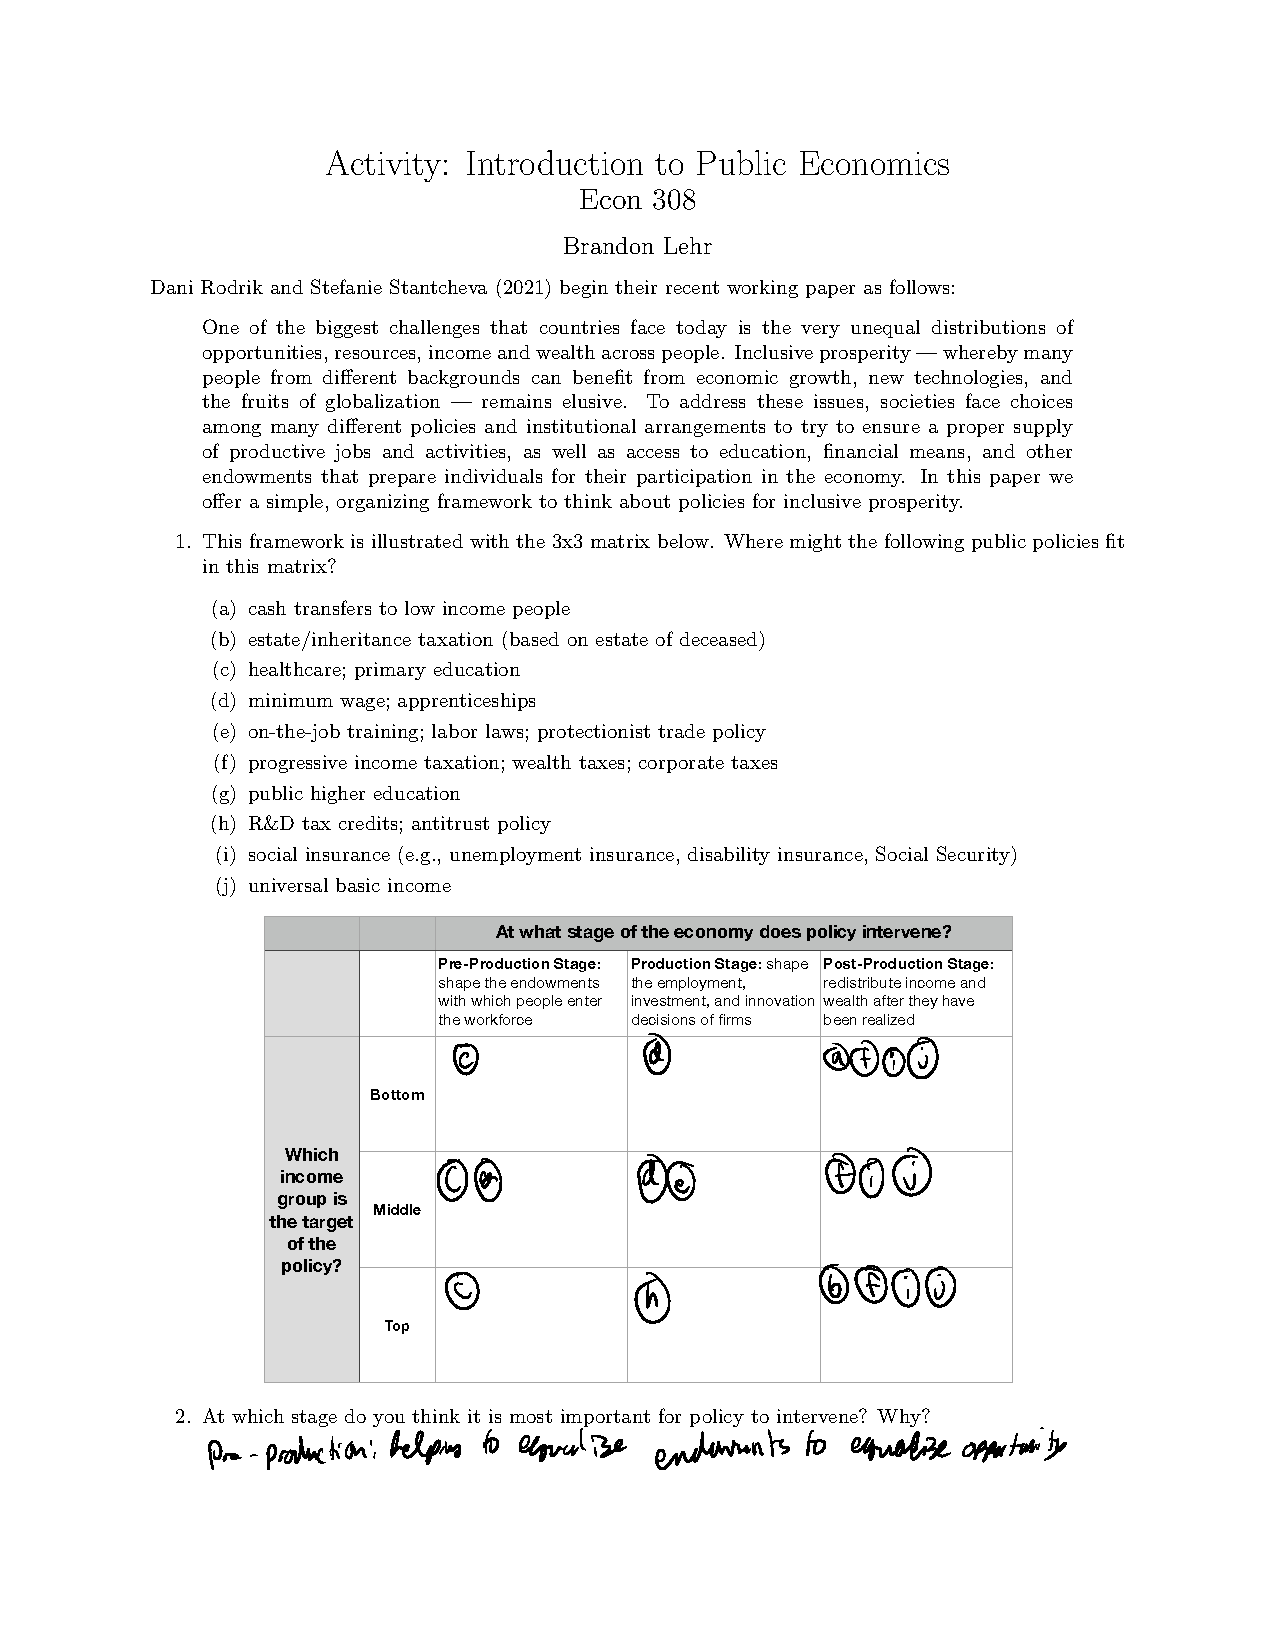
\includegraphics[width=\textwidth]{Activity_1.pdf}
      \end{center}
    \end{problem}
  \end{problem}
}\end{document}
